\chapter{The Standard Model}
Everything this thesis is built on has its roots in the Standard Model (SM). The Standard Model of particle physics addresses the question \emph{What is matter made of?} on the smallest possible scale. It links the fundamental constituents of the universe together along with the forces that bind them, in order to describe and predict the laws of nature. The Standard Model is formulated as a quantum field theory, where the fundamental particles are spin-1/2 fermions which interact with one another through the exchange of spin-1 gauge bosons. These interactions come in three forms, mediated by three different types of gauge bosons: The electromagnetic force, mediated through photons; the weak force, mediated through W and Z bosons; and the strong force, mediated by gluons. How the fundamental particles interact also defines which properties they exhibit. In addition, the Standard Model includes a field very different from the others, the Higgs field. The Higgs field interacts with both fermions and bosons and is what gives all particles their mass.\newline
One thing the Standard Model fails to incorporate is the force of gravity. This shortcoming is one of the main motivations for looking for alternative models beyond the Standard Model (BSM), which is the main topic of this thesis.

\section{Fundamental particles: quarks and leptons}
It appears that all matter in the universe can be described by a very small collection of fundamental particles, six leptons and six quarks. These are collectively called fermions and are, as far as we can tell, truly elementary (not composed of any other particles).
Leptons are particles with integer or zero electric charge, defined in units of electron charge. They come in three flavors, or generations, and their mass increases with generation. Each generation of leptons consists of two particles: one charged lepton and one neutrally charged particle denoted as \emph{neutrino ($\nu$)}. The three generations can be arranged in a doublet structure, and are as follows.
\begin{equation}
\label{eqn:lepton_flavor_doublets}
\begin{pmatrix} \nu_e      \\ e      \end{pmatrix} \qquad
\begin{pmatrix} \nu_{\mu}  \\ \mu    \end{pmatrix} \qquad
\begin{pmatrix} \nu_{\tau} \\ \tau   \end{pmatrix}
\end{equation}
The charged leptons can be positively or negatively charged, defined in units of electron charge $e$. By convention the leptons of matter are negatively charged, $e^{-}$, $\mu^{-}$, and $\tau^{-}$,  whereas the positively charged leptons,  $e^{+}$, $\mu^{+}$, and $\tau^{+}$ are considered their anti-particles.
% Each lepton generation is assigned its own quantum number $L$ which must be conserved after any process.
A summary of the lepton properties is listed in Table~\ref{table:theory:lepprop}.
\begin{table}[h!]
\begin{center}
\begin{tabular}{|c|c|c|}% c c c|}
\hline
Lepton        & Mass           & Charge \\%& $L_{e}$ & $L_{\mu}$ & $L_{\tau}$ \\
\hline
$e^{-}$      & $0.51 \mbox{ MeV}$      & $e$ \\%& 1       & 0         & 0 \\
$\mu^{-}$    & $105.7 \mbox{ MeV}$      & $e$ \\%& 0       & 1         & 0 \\
$\tau^{-}$   & $1776.9 \mbox{ MeV}$     & $e$ \\%& 0       & 0         & 1 \\
\hline                                      
$\nu_{i}$, $i=e,\mu,\tau$ & $\sum_i m_i < 0.170 \mbox{ eV}$       & $0$ \\%   & 1       & 0         & 0 \\
% $\nu_{\mu}$  & $< 0.19 \mbox{ MeV}$   & $0$ \\%   & 0       & 1         & 0 \\
% $\nu_{\tau}$ & $< 18.2 \mbox{ MeV}$   & $0$  \\%   & 0       & 0         & 1 \\
\hline
\end{tabular}
\end{center}
\caption{Lepton Properties~\cite{Patrignani:2016xqp,refId0}.}
\label{table:theory:lepprop}
\end{table}
Leptons interact with one another through the \emph{electromagnetic and weak forces}, which will be explained in more detailed in Section~\ref{sec:theory:ew}.\newline
The other six fundamental particles of matter are the \emph{quarks}. They are distinguished from the leptons in that they, in addition to interacting through the weak and electromagnetic forces, interact with one another through the \emph{strong force}, described in Section~\ref{sec:theory:qcd}. This force binds the quarks together to form baryons (like protons and neutrons) or mesons (like pions), and in addition, keeps the quarks from being observed as free particles such that they are only visible through their baryon or meson bound states (commonly referred to as \emph{hadrons}). Also organized in three generations, the six quarks are called \textit{up}, \textit{down}, \textit{charm}, \textit{strange}, \textit{top} and \textit{bottom}, and are organized in flavor doublets as follow
\begin{equation}
\label{eqn:quark_flavor_doublets}
\begin{pmatrix} u \\ d \end{pmatrix} \qquad
\begin{pmatrix} c \\ s \end{pmatrix} \qquad
\begin{pmatrix} t \\ b \end{pmatrix}
\end{equation}
Each quark comes with a fractional charge of $\frac{2}{3}$ (u, c and t) and $-\frac{1}{3}$ (d, s and b) of one electron charge. As with the leptons, there are also distinct particles of opposite charge, anti-quarks. Some of the quark properties are listed in Table~\ref{table:theory:quarkprop}.
\begin{table}
\begin{center}
\begin{tabular}{|c|c|c|}%c|}
\hline
Quark & Mass & Charge \\% & Properties \\
\hline
u & $1-5 \mbox{ MeV}$         & $\phantom{-}\frac{2}{3} e$  \\%& $I_{z} = \frac{1}{2}$ \\
d & $3-9 \mbox{ MeV}$         & $-\frac{1}{3} e$            \\%& $I_{z} = -\frac{1}{2}$ \\
c & $1.15-1.35 \mbox{ GeV}$   & $\phantom{-}\frac{2}{3} e$  \\%& Charm = +1 \\
s & $75-170 \mbox{ MeV}$      & $-\frac{1}{3}e$             \\%& Strangeness = -1 \\
t & $172.4\pm 0.1 \mbox{ GeV}$ & $\phantom{-}\frac{2}{3} e$  \\%& Top = +1 \\
b & $4.0-4.4 \mbox{ GeV}$     & $-\frac{1}{3} e$            \\%& Bottom = -1 \\
\hline
\end{tabular}
\end{center}
\caption{Quark Properties}
\label{table:theory:quarkprop}
\end{table}
\par These 12 fermions, together with their corresponding anti-particles, represent the fundamental particles of the universe and constitute all matter around us. There are four fundamental forces that we know of: gravity, electromagnetism, the weak force and the strong force. Gravity is extremely weak compared to the other forces and we currently lack a quantum field theory of its interaction, therefore it is typically ignored in high energy physics experiments. 
All particles that are electrically charged, the charged leptons ($e$, $\mu$ and $\tau$) and all of the quarks, interact through the electromagnetic force. These interactions are governed by the laws of Quantum Electrodynamics (QED), and are mediated through the massless and electrically neutral spin-1 photon. All of the fermions, including the electrically neutral neutrinos, feel the weak force and undergo weak interactions. The weak force is mediated through the vector bosons $\PW^+$, $\PW^-$ and $\PZ^0$, which are heavy charged particles with a spin of 1. Finally, there is the strong force, mediated by the massless and electrically neutral spin-1 gluon. Only quarks interact via the strong force, and it is that interaction that makes the quarks so fundamentally different from leptons and neutrinos. Their interaction is governed by the laws of Quantum Chromodynamics (QCD). All of these interactions can be represented in one common gauge theory, the Standard Model.

\section{The Standard Model Lagrangian}
\label{sec:theory:gauge}
The Standard Model is a quantum gauge field theory in which each particle is described as a dynamical field with a value at each space-time coordinate. These fields are governed by a Lagrangian density function, the Standard Model. For instance, the Lagrangian density of a free fermion, one not interacting with any other fields, is
\begin{equation}
  \label{eq:theory:freeLag}
  \mathcal{L} = \bar{\Psi}(x^{\mu})(i\lambda^{\mu}\partial_{\mu}-m)\Psi(x^{\mu})
\end{equation}
where $\Psi(x^{\mu})$ represents any spin-1/2 fermion field, also called \emph{Dirac field}, as a function of space-time; $\bar{\Psi}=\Psi^{\dagger}\gamma_0$, where $\gamma^0$ is one of the gamma matrices $\gamma^{\mu}$ and is included in order to make $\Psi^{\dagger}\Psi$ invariant under Lorentz transformation; and $m$ is the mass of the fermion in question. Any interaction between the fundamental particles due to the fundamental forces, can be described as variations in the Lagrangian of quantum fields and are represented as additional terms in the equation above.\par
Being a gauge theory, the Standard Model has the property of gauge invariance, meaning that measurable quantities stay the same despite the fields themselves changing. If observables stay the same after a field transformation, there is a symmetry in the system. The symmetries of the Standard Model arise due to the fact that fermions of a given type are indistinguishable from one another. These symmetries result in the presence of \emph{force mediators}, which arise as a representation of infinitesimal generators of some symmetry group.
 %The spin-1/2 fermion fields are arranged in \emph{Weyl spinors}, listen in Equation~\ref{eqn:lepton_flavor_doublets} and~\ref{eqn:quark_flavor_doublets}, which transform differently depending on their quantum numbers. 
The fermion fields can be arranged as particle multiplets where one transforms into the other under a symmetry transformation. A symmetry transformation produce rotations between the particles of a given multiplet, but never to a field outside of that group. The symmetry group of the Standard Model is the direct product
\begin{equation}
  SU(3)_C \otimes SU (2)_L \otimes U(1)_Y.
\end{equation}
$SU(3)_C$ is the color ($C$) symmetry allowing the rotation of quarks, arranged in color multiplets, into one another, corresponding to interactions produced by the strong force. The colors are denoted as red, green and blue. $SU (2)_L \otimes U(1)_Y$ represent the electroweak force with weak left-handed isospin $L$ and weak hypercharge $Y$ symmetries, acting on $L$ and $Y$ multiplets, respectively. %These forces, together with their conserved charges, will be clarified in the sections below.
The particle multiplets of the Standard Model can then be written as $\mathcal{G}_{SM} \ni x=(C,L)_{(Y)}$ and are (for illustrations only for the the 1st generation):
\begin{alignat}{3}
  \label{eq:theory:multiplets}
Q &= (3,2)_{(1/3)} &&=
  \begin{pmatrix} 
    u_r & u_g & u_b \\
    d_r & d_g & d_b
    \end{pmatrix} \quad  &&\sim \textrm{quark multiplet} \\[1pt]
L &= (1,2)_{(-1)} &&= \begin{pmatrix} \nu_e & e \end{pmatrix} \quad &&\sim \textrm{leptonic doublet} \\[1pt]
u^c &= (\bar{3},1)_{(-4/3)} &&= \begin{pmatrix} u_{\bar{r}}^c & u_{\bar{g}}^c & u_{\bar{b}}^c\end{pmatrix} \quad &&\sim \textrm{anti-up quarks} \\[1pt]
d^c &= (\bar{3},1)_{(2/3)}  &&= \begin{pmatrix} d_{\bar{r}}^c & d_{\bar{g}}^c & d_{\bar{b}}^c\end{pmatrix} \quad &&\sim \textrm{anti-down quarks} \\[1pt]
e^c &= (1,1)_{(2)}          && \quad &&\sim \textrm{positron} \\
\end{alignat}
The right-handed neutrino (which in needed to generate a Dirac mass for the neutrinos) is not included here because it is a SM \emph{singlet} and does not transform under the SM group $\mathcal{G}_{SM}$, but it could be written as $\nu^c=(1,1)_{(0)}$. The positron $e^c$, on the other hand, \emph{is} included as its hypercharge is non-zero and it therefore undergoes $U(1)_Y$ interactions. These five multiplets exist for each of the three generations.\newline
The numbers representing each multiplet correspond to which representation it belongs to. For instance, we see that the quark multiplet transforms as a triplet under $SU(3)_C$, a doublet under $SU(2)_L$ and has a non-zero hypercharge, corresponding to a non-trivial representation under $U(1)_Y$. That corresponds to saying that quarks interact through all of the three fundamental interactions. From that notation, it is also clear that leptons do not carry color charge, and will only interact via the electroweak interactions.\newline
From the multiplets above, we see that $u^c$ and $d^c$ transform as singlets under $SU(2)_L$, meaning they do not interact. This, however, does not mean they do not feel the electroweak force. The electroweak gauge bosons \PW and \PZ are not directly part of $SU(2)_L$, rather, they are a linear combination of $SU(2)_L$ and $U(1)_Y$ and anything with a non-zero weak hypercharge $Y$ will interact with them. This is also true for the photon, which also is a linear combination of $SU(2)_L$ and $U(1)_Y$. These interactions; the strong, weak and electromagnetic, will be explained in more detail in the following sections.

\subsection{The quantum chromodynamics sector}
\label{sec:theory:qcd}
The group $SU(3)_C$ describes the strong interaction mediated by gluons, and is described by the quantum gauge theory Quantum Chromodynamics (QCD). The group is generated by 8 linearly independent matrices $T^a=\frac{\lambda^a}{2}$, where $\lambda^a$ are the Gell-Mann matrices~\cite{PhysRev.125.1067}. The generator matrices do not commute with one another, but rather satisfy the commutation relation $[\lambda^i/2,\lambda^j/2]=i f^{ijk} \lambda_k/2$. This property makes the $SU(3)_C$ group \emph{non-Abelian}, which consequently results in the gluons themselves being charged and displaying self-interactions. Gluons are charged with one unit of color and one unit of anti-color. Quarks, the only fundamental particles interacting with the strong force, are arranged in the simplest representation of $SU(3)$ and come with one unit of color or anti-color. \par
The generators are collectively referred to as the \emph{group representation} of $SU(3)_C$. Any group element can be can be written as $e^{-i\theta^a g_a}$, where $a$ runs from 1 to 8, $\theta^a$ are real numbers and $g_a$ represent one of the eight linearly independent $\lambda/2$ matrices (generators). Given one representation, one can always find another one through any local gauge transformation that leaves the commutator unchanged.  
In this case, the group elements are the quark fields, and a local gauge transformation of fields becomes
\begin{equation}
  \Psi(x^{\mu}) \rightarrow e^{ -i g_s \theta^a(x^{\mu}) T^a}\Psi(x^{\mu}),
\end{equation}
where $g_s$ is the strong coupling, $\theta^a(x^{\mu})$ some arbitrary function and $a$ runs over the eight generators of the group. In order to keep the Lagrangian in Equation~\ref{eq:theory:freeLag} invariant under such a transformation, an additional term must be added, replacing the partial derivative $\partial_{\mu}$ with the \emph{covariant derivative}
\begin{equation}
  D_\mu=\partial_\mu + ig_s \mathcal{A}_{\mu}^a T^a ,
\end{equation}
introducing a tensor $\mathcal{A}_{\mu}^a$ that represents the 8 gluon fields.
The QCD Lagrangian then becomes
\begin{equation}
  \label{eq:theory:qcdl}
   \mathcal{L}_{QCD} =-\frac{1}{4}{\cal F}_{a}^{\mu\nu}{\cal F}^{a}_{\mu\nu}+\bar{\Psi}(x^{\mu})(i\lambda^{\mu}D_{\mu}-m)\Psi(x^{\mu}),
\end{equation}
where $F_{\mu\nu}^a$ is the gauge field of the group, the gluon field tensor 
\begin{equation}
F_{\mu\nu}^a=\partial_{\mu} \mathcal{A}_{\nu}^a-\partial_{\nu} \mathcal{A}_{\mu}^a+g_s f^{abc}\mathcal{A}_{\mu}^b\mathcal{A}_{\nu}^c.
\end{equation}
The first term in Equation~\ref{eq:theory:qcdl} represents the quark-gluon interaction, leading to vertices like the one on the left in Figure~\ref{fig:theory:qcdint}. The second, the gluon field kinetic term, picks up the \emph{structure constant} $f^{abc}$ due to the commutation relation of the $\lambda$ matrices. This term creates self-interactions between the gluon fields, like the two shown on the right in Figure~\ref{fig:theory:qcdint}.
\begin{figure}[h!]
\centering
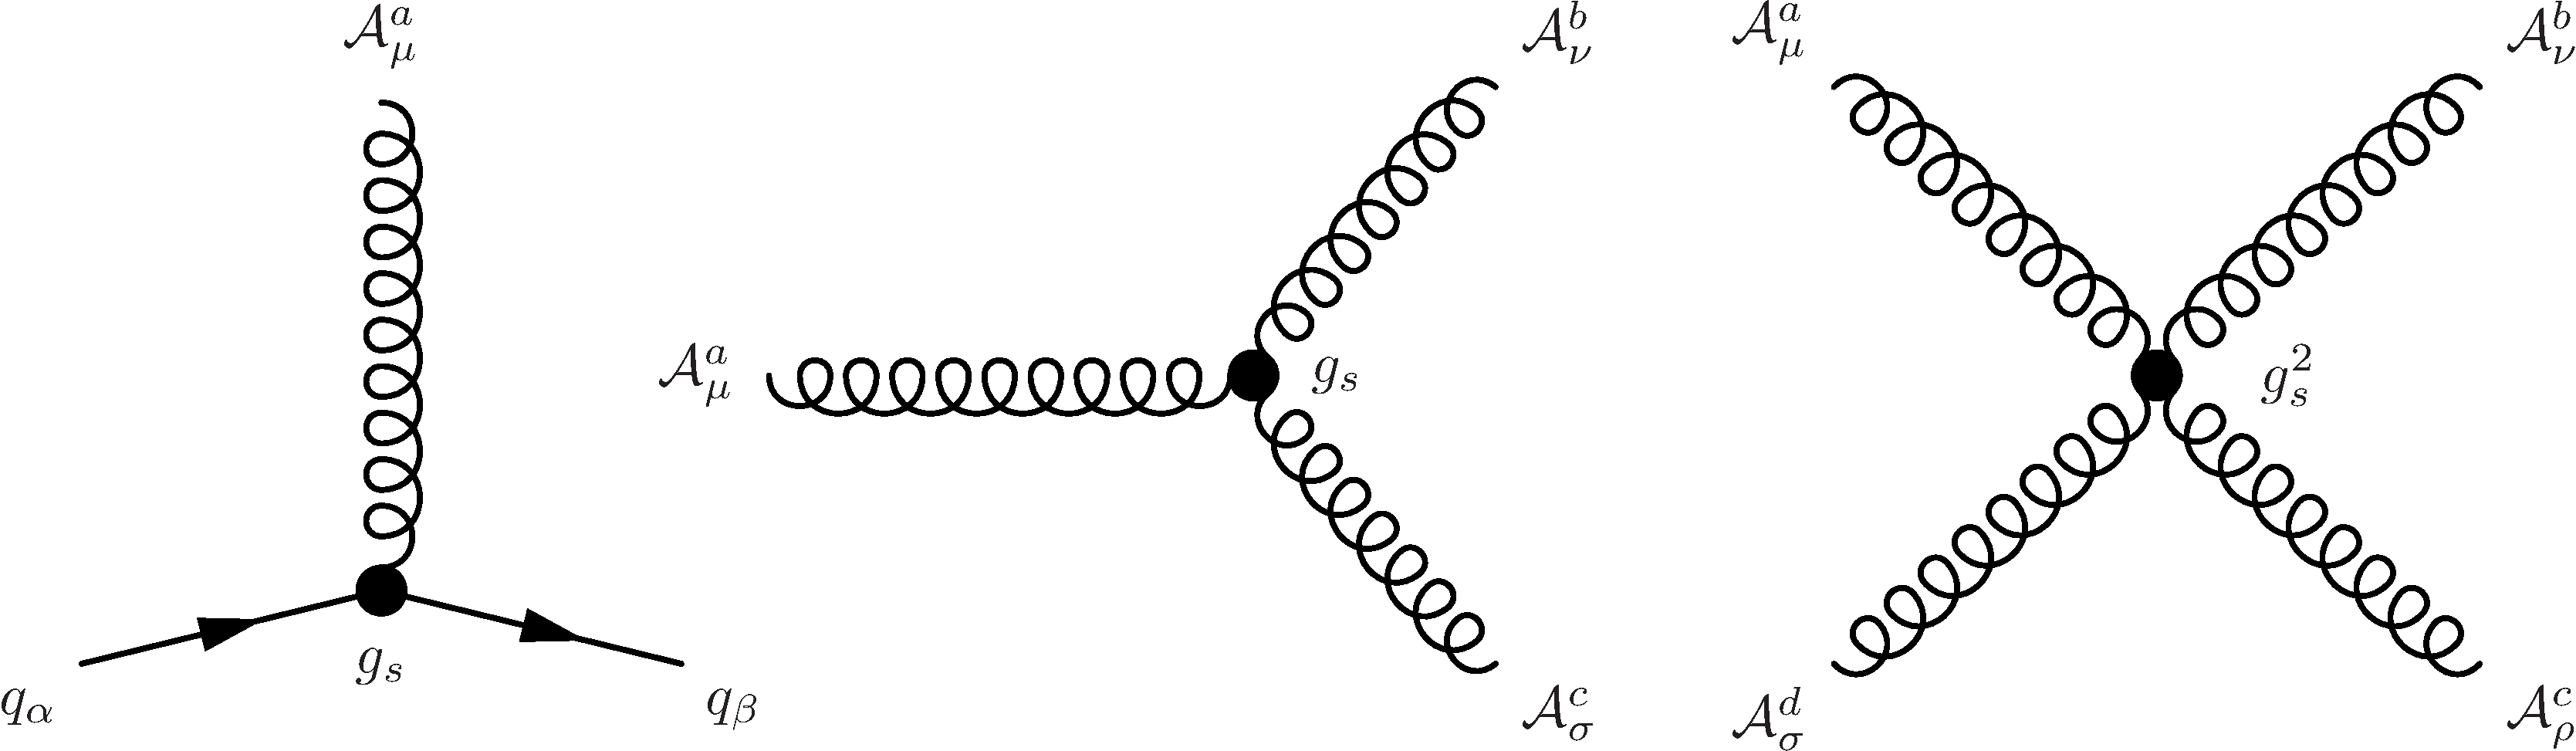
\includegraphics[width=0.79\textwidth]{figures/theory/QCD_vtx.pdf}
\caption{The QCD interaction vertices: quark interaction with the gluon field (left), and three-gluon (middle) and four-gluon (right) self-interaction vertices.}
\label{fig:theory:qcdint}
\end{figure}
These self-interactions have severe consequences: any bare color charge, like a quark, will be surrounded by a sea of virtual gluons and quarks that share the same color. When probing the quark color at higher and higher energies, corresponding to shorter and shorter distances, the color charge decreases until only the bare charge is visible. There, the quarks are essentially free and can be observed as distinguishable particles. This property is referred to as \emph{asymptotic freedom}. For the same reasons, when going further and further away from a bare color charge, the sea of charges surrounding it makes the observed charge increase. That results in a strong attractive force between color charges at large distances, where the potential energy between the two grows linearly with the distance between them as
\begin{equation}
  V(r)=-\frac{4\alpha_s}{3r}+kr,
\end{equation} 
where $r$ is the distance between the quarks and $\alpha_s$ is the coupling strength of QCD.
%, describing how the observed charge between two quarks increases depending on the distance between them. 
When the distance between the quarks grows very large, this potential energy is enough to create real quark-antiquark pairs from the vacuum in order to reduce the potential energy, a process called \emph{fragmentation}. Whenever one tries to separate quarks form one another they will fragment, which consequently means that quarks are never observed on their own. Rather, they form colorless (uncharged under the color charge) bound states of mesons or baryons (collectively called hadrons), a property called \emph{color confinement}. The energy for which the confinement into hadrons occurs, also called \emph{hadronization}, is defined through experimental measurement and found to be $\Lambda_{QCD}=100-500 \MeV$ (around the mass of the lightest hadrons). The effective charge between the quarks, $\alpha_S$, changes as a function of energy as
 \begin{equation}
   \alpha_S(Q)=-\frac{6\pi}{33-2n_f}\ln(Q/\Lambda_{QCD})
 \end{equation}
where $Q$ is the energy of the probe used to measure the charge and $n_f$ is the number of quark flavors (u, d, c, s, b, t) at that energy. The value $\alpha_S$ is around 0.1 for energies between 100-1000 \GeV.

\subsection{The electroweak sector}
\label{sec:theory:ew}
The electromagnetic and weak interactions arise from the breaking of $SU (2)_L \otimes U(1)_Y$ symmetry. While the unification of the electromagnetic and weak force is obtained under the $SU (2)_L \otimes U(1)_Y$ group, the predicted gauge bosons of such a group are not observed in nature: three charged massless vector bosons and one neutral massless boson. Rather, the $\PW^{\pm}$, $\PZ^{0}$ and the photon arise from the spontaneous symmetry breaking of $SU (2)_L \otimes U(1)_Y$ to $U(1)_{EM}$. This happens due to the \emph{Higgs mechanism}, and exactly how this occurs will be the topic of Section~\ref{sec:theory:higgs}.\par
The symmetry under $SU (2)_L$ is called weak left-handed isospin $L$, and the symmetry under $U(1)_Y$ is the weak hypercharge $Y$. The name "left-handed" arise from the fact that \emph{parity} is violated in the electroweak interactions. All the fundamental fermions have a \emph{chirality}, defined as the projection of the particles spin along its direction of motion. Charged weak interactions are only observed for fermions of left-handed chirality (vector minus axial coupling, V-A). While the left-handed fermion fields are in the simplest doublet representation of $SU(2)$ with weak isospin $I=1/2$, the fermions of right-handed chirality are therefore in the singlet representation with weak isospin $I=0$, meaning they do not interact with the gauge bosons of $SU (2)_L$. The chirality of any fermion $\Psi$ can be defined through the operator $\gamma^5$, the product of the four Dirac matrices~\cite{Pauli:1936gd} $\gamma^5=i\gamma^1\gamma^2\gamma^3\gamma^4$. Any fermion field can be projected into its chiral components $\Psi_L$ or $\Psi_R$ through the projection operation
\begin{equation}
  \Psi_L = \frac{1-\gamma^5}{2} \quad \textrm{and} \quad \Psi_R = \frac{1+\gamma^5}{2}.
  \end{equation}
The gauge field tensor of the group of $SU (2)_L$ symmetry is $W_{\mu\nu}^a$, where $a$ runs over the 3 generators of the group. The conserved charge associated with the group is the \emph{third} component of weak isospin $I_3$, and all weak interactions must preserve $I_3$. The generators of the group are defined as $T_i=\frac{\sigma_i}{2}$, where $\sigma_i$ are the Pauli matrices~\cite{inbook}. As for $SU (3)_C$, the group is non-abelian and the generators follow the commutation relation $[\sigma_i/2,\sigma_j/2]=i \epsilon_{ijk} \sigma_k/2$, where $\epsilon_{ijk}$ is the Levi-Civita permutation symbol~\cite{Duplij2004}. This in turn implies self-interactions between the gauge bosons of the group. The latter group, $U(1)_Y$ of weak hypercharge $Y$, is abelian and hence displays no self-interaction. The gauge field tensor $B_{\mu\nu}^a$ interacts with both left- and right-handed fermion fields. Similar to the case for QCD, a local gauge transformation of $SU (2)_L \otimes U(1)_Y$ requires the addition of additional terms in the derivate in order to keep the Lagrangian invariant. The partial derivative $\partial_{\mu}$ is replaced by the covariant derivatives
\begin{align}
  \label{eq:theory:ewcov}
  D_\mu \Psi_L &=(\partial_{\mu} + ig_2 T_a W_{\mu}^a + ig_1 \frac{Y}{2} B_{\mu}^a)\Psi_L\\
  D_\mu \Psi_R &=(\partial_{\mu} + ig_1 \frac{Y}{2} B_{\mu}^a)\Psi_R.
\end{align}
After the substitution, the electroweak Lagrangian can be written as a sum of four terms:
\begin{equation}
  \label{eq:theory:ewl}
   \mathcal{L}_{EW} = \mathcal{L}_{gauge}+\mathcal{L}_{f}+\mathcal{L}_{Yukawa}+\mathcal{L}_{\phi}.
\end{equation}
\par The first term, $\mathcal{L}_{gauge}$, represent the kinetic field tensor and is
\begin{equation}
  \label{eq:theory:gauge}
   \mathcal{L}_{gauge} = -\frac{1}{4}W_{a}^{\mu\nu}W^{a}_{\mu\nu} - \frac{1}{4}{\cal B}^{\mu\nu}{\cal B}_{\mu\nu}
\end{equation}
where the gauge field tensors are
\begin{align}
W_{\mu\nu}^a &=\partial_{\mu} W_{\nu}^a-\partial_{\nu} W_{\mu}^a-g_2\epsilon^{ijk}W^{j}_{\mu}W^{k}_{\nu} \quad \textrm{, with   } i=1-3\textrm{ and}\\
B_{\mu\nu} &=\partial_{\mu} B_{\nu}-\partial_{\nu} B_{\mu}.
\end{align}
The non-abelian nature of $SU (2)_L$ leads to trilinear and quadrilinear couplings between the photon and vector bosons as illustrated in Figure~\ref{fig:theory:weakint}.
\begin{figure}[h!]
\centering
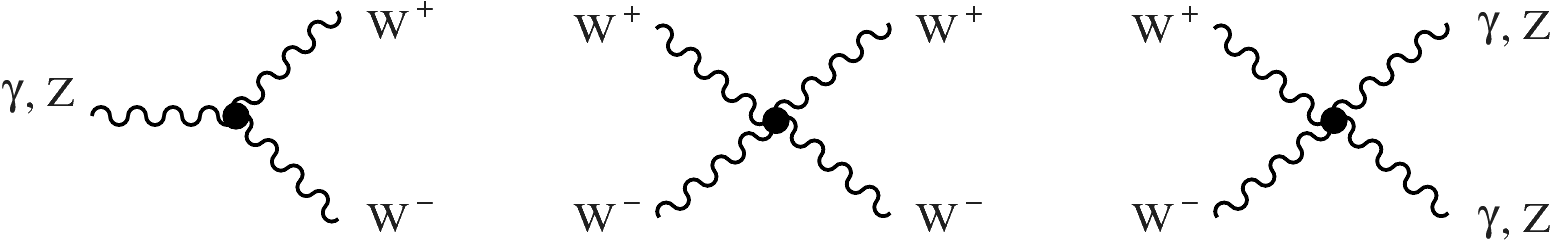
\includegraphics[width=0.99\textwidth]{figures/theory/weak_selfinteraction.png}
\caption{The electroweak self-interaction vertices: trilinear (left), and quadri-linear (middle and right) vertices.}
\label{fig:theory:weakint}
\end{figure}
\par The second term describe the boson fields coupling to fermions and is
\begin{equation}
  \label{eq:theory:gauge}
   \mathcal{L}_{f} = \bar{Q}_ii\lambda^{\mu}D_{\mu} Q_i + \bar{u}_i^ci\lambda^{\mu}D_{\mu} u_i^c
                   + \bar{d}_i^ci\lambda^{\mu}D_{\mu} d_i^c + \bar{L}_ii\lambda^{\mu}D_{\mu} L_i +  
                     \bar{e}_i^ci\lambda^{\mu}D_{\mu} e^c_i,
\end{equation}
where we have expressed each term using the particle multiplets in Equation~\ref{eq:theory:multiplets} and the subscript $i$ runs over the three fermion generations. They all interact differently under $SU(2)_L \times U(1)_Y$ due to their different charges.\newline
Up until now we have considered the Lagrangian before spontaneous symmetry breaking, where we have three charged massless bosons and one massless neutral boson, a constellation we know to be wrong from observations. When I have referred to interaction vertices, I have loosely referred to W, Z and $\gamma$ vertices without explicitly defining them. We will show in Section~\ref{sec:theory:higgs} that, due to spontaneous symmetry breaking, the charged gauge boson fields $\PW^{\pm}$ in reality are linear combinations of $W_{\mu}^1$ and $W_{\mu}^2$ given as
\begin{equation}
\PW^{\pm} = \frac{1}{\sqrt{2}}(W_{\mu}^1 \mp iW_{\mu}^2).
\end{equation}
These are responsible for \emph{charged-current interactions}, which turn up-type fermions into their corresponding down-type fermions within the same generation, and vice-versa. The electrically neutral Z boson and the photon fields are expressed in terms of $W_{\mu}^3$ and $B_{\mu}$ through the weak mixing angle~\cite{Weinberg:1979pi} as
\begin{equation}
\begin{pmatrix} \gamma \\ \PZ^0 \end{pmatrix}
  = \begin{pmatrix} \cos \theta_W & \sin \theta_W \\
                   -\sin \theta_W & \cos \theta_W \end{pmatrix}
  \begin{pmatrix} B \\ W^3 \end{pmatrix}                   
\end{equation}
where $\theta_W$ can be expressed through the $SU (2)_L$ and $U(1)_Y$ couplings $g_1$ and $g_2$ as
\begin{equation}
     \cos \theta_W = \frac{g_1}{g^2_1+g^2_2}  \quad \textrm{ and } \quad \sin \theta_W = \frac{g_2}{g^2_1+g^2_2}.        
\end{equation}
The electric charge is defined through weak isospin and hypercharge, and is
\begin{equation}
  Q = I_3 + \frac{Y}{2}.
  \end{equation}
A few of the fermion-boson vertices are shown in Figure~\ref{fig:theory:weakfermionint}.\par
  \begin{figure}[h!]
  \centering
  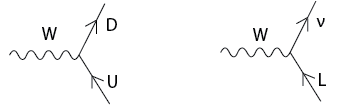
\includegraphics[width=0.45\textwidth]{figures/theory/ew_ch.png}\\
  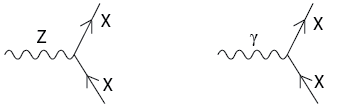
\includegraphics[width=0.45\textwidth]{figures/theory/ew_neu.png}
  \caption{The electroweak fermion interaction vertices. Top: charged-current interaction vertex connecting a charged vector boson $\PW^{\pm}$ to quarks (left) and leptons (right). Bottom: neutral-current interactions between the neutral $\PZ^0$ boson and any fermion (left), and between a $\gamma$ and electrically charged fermions.}
  \label{fig:theory:weakfermionint}
  \end{figure}
The last two terms, $\mathcal{L}_{Yukawa}$ and $\mathcal{L}_{\phi}$, are related to the Higgs boson and represent couplings to the Higgs field: the Yukawa interaction term which generates masses for the fermions due to the non-zero Higgs vacuum expectation value, and the Higgs bosons interactions with itself and with the gauge bosons. Introduced as an extension to the original Standard Model, the Higgs sector is one of the greatest accomplishments of particle physics in the 20th century and one of the reasons why the LHC was built. How it arises is what we will turn to next.

\subsection{The Higgs sector}
\label{sec:theory:higgs}
The problem of having massless gauge bosons under $SU(2)_L \times U(1)_Y$, while observing massive W and Z bosons, was independently solved by three different groups and has become known as the Englert–Brout-Higgs–Guralnik–Hagen–Kibble mechanism of spontaneous symmetry breaking~\cite{PhysRevLett.13.321,PhysRevLett.13.508,PhysRevLett.13.585}, an accomplishment for which Peter Higgs and Francois Englert shared the 2013 Nobel Prize.\newline
It began with the realization that the breaking of a local gauge symmetry could give rise to a final mass for the gauge boson involved. This was first discovered in association with superconductivity, where it was found that when a normal metal becomes superconducting the photon field inside the superconductor would acquire a finite mass~\cite{PhysRev.110.827}.

\subsubsection{Spontaneous breaking of a global gauge symmetry}
In order to achieve spontaneous symmetry breaking, Jeffrey Goldstone~\cite{Goldstone:1961eq} suggested introducing a massive complex scalar field $\phi$ with quantum numbers of the vacuum and then giving the field a vacuum expectation value. The field
\begin{equation}
\phi = \frac{1}{\sqrt{2}}(\phi_1+i\phi_2)  
\end{equation}
would have a Lagrangian of the form
\begin{equation}
\mathcal{L} = \partial^{\mu}\bar{\phi}\partial_{\mu}\phi-\mu_0^2\bar{\phi}\phi-\frac{\lambda_0}{6}(\bar{\phi}\phi)^2,
\end{equation}
where $\lambda_0$ is the coupling constant and $\mu_0$ is the mass. The Lagrangian is invariant under $U(1)$, though in this case under a global symmetry and not a local one. If one takes $\mu_0^2$ to be negative, the potential will get a minima along a circle of radius $v$ such that
\begin{equation}
  \phi_1^2+\phi_2^2 = v^2 \quad \textrm{and}\quad v^2=\frac{\mu_0^2}{\lambda_0},
\end{equation}
and take the form of a "Mexican Hat" as shown in Figure~\ref{fig:theory:higgspot}. 
  \begin{figure}[h!]
  \centering
  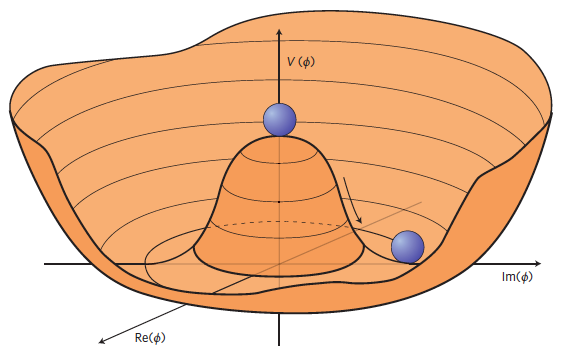
\includegraphics[width=0.49\textwidth]{figures/theory/higgspotential.png}
  \caption{The potential $V(\phi)$ for a complex scalar field with $\mu_0^2<0$~\cite{Ellis:1638469}.}
  \label{fig:theory:higgspot}
  \end{figure}
The variable $v$ is referred to as the vacuum expectation value (VEV). The lowest value of the Hamiltonian is now at $\phi=v$ rather than at $\phi=0$. Goldstone then translated the field to a minimum energy position $\phi'=\phi+v$ and gave the field a vacuum expectation value, effectively breaking the symmetry between the two field components, but keeping the Lagrangian invariant.
This complex field can be expanded around the ground state in terms of two real fields $\eta$ and $\epsilon$ that represent deviations from the minimum:
\begin{equation}
\phi(x) = \frac{1}{\sqrt{2}}*(v+\eta(x)+i\epsilon(x))
\end{equation}
 The Lagrangian then becomes
\begin{equation}
\mathcal{L} = \frac{1}{2}(\partial_{\mu}\epsilon)^2 + \frac{1}{2}(\partial_{\mu}\eta)^2+\mu_0^2\eta^2 + \textrm{ additional terms}.
\end{equation}
The third term has the form of a mass term for the scalar $\eta$ field. However, the $\epsilon$ field has no mass term, meaning that the theory contains a massless scalar, referred to as a \emph{Goldstone boson}. This is expressed through \emph{Goldstone's theorem}, which states that whenever a continuous symmetry of a physical system is spontaneously broken, massless scalars will occur. Rather than providing a mass term for the vector bosons, the theory acquired one massive scalar and one massless scalar not observed in nature, requiring the gauge theory of weak interactions to look for solutions elsewhere.

\subsubsection{The Higgs mechanism}
The solution to the problem came a few years later, in 1964, when spontaneous symmetry breaking of a \emph{local} gauge symmetry was studied gather than a global. For a $U(1)$ symmetry, this requires the Lagrangian to be invariant under $\phi \rightarrow e^{i\theta(x)}\phi$, with the derivative replacement
\begin{equation}
D_{\mu}=\partial_{\mu}-ie A_{\mu}.
\end{equation}
After translating the field $\phi$ to its true ground state and writing out the Lagrangian,
\begin{equation}
  \label{eq:theory:higgsL}
\mathcal{L} = \frac{1}{2}(\partial_{\mu}\epsilon)^2 + \frac{1}{2}(\partial_{\mu}\eta)^2-v^2\lambda \eta^2+\frac{1}{2}v^2 e^2 A_{\mu} A^{\mu}-ev, A_{\mu}\partial^{\mu}\epsilon-\frac{1}{4}F_{a}^{\mu\nu}F^{a}_{\mu\nu}
\end{equation}
we see that the particle spectrum now contains a massless Goldstone boson $\epsilon$, a massive scalar $\eta$ and, finally, a massive vector $A_{\mu}$ with $m_A=ev$. Despite the success of having dynamically created the mass for the gauge field, one had to tackle the problem of the massless scalar. The solution was found through the realization that one of the fields was unphysical; by giving mass to the vector $A_{\mu}$, the polarization degrees of freedom had increased from 2 to 3 through adding a longitudinal polarization. However, this should not be possible when simply translating field variables. It was found that through a simple gauge transformation with a different set of fields
\begin{equation}
A_{\mu} \rightarrow A_{\mu}+\frac{1}{ev}\partial_{\mu}\theta,
\end{equation}
the Goldstone boson would disappear and turn into the longitudinal polarization of the massive gauge boson and that the theory was left with one massive vector gauge boson, $A_{\mu}$, and another massive scalar, $h$. This is what is referred to as the \emph{Higgs mechanism}.

\subsubsection{The Weinberg-Salam Model}
The final step is to formulate the Higgs mechanism such that the vector bosons $\PW^{\pm}$ and $\PZ^{0}$ become massive, while the photon remains massless. To do so Sheldon Glashow, Abdus Salam, and Steven Weinberg (all awarded the 1979 Nobel Prize for electroweak unification), added a gauge-invariant term to the electroweak Lagrangian of the following form:
 \begin{align}
   \label{eq:theory:higgsmass}
  \mathcal{L}_{Higgs}= \big|(i\partial_{\mu} - g_2 T_a W_{\mu}^a -vg_1 \frac{Y}{2} B_{\mu}^a) \phi\big| ^2-V(\phi).
 \end{align}
The $\phi_i$ has to belong to $SU(2) \times U(1)$ multiplets, and the simplest configuration corresponds to four fields in an isospin doublet of weak hypercharge $Y=1$:
\begin{equation}
\phi =  \begin{pmatrix} \phi^{+} \\ \phi^{0} \end{pmatrix}= \begin{pmatrix} \frac{\phi_1+i\phi_2}{\sqrt{2}} \\ \frac{\phi_3+i\phi_4}{\sqrt{2}}\end{pmatrix}.
\end{equation}
To generate the necessary masses, the Higgs potential from the previous section is used, with a vacuum expectation value of
\begin{equation}
\phi_0 = \frac{1}{\sqrt{2}}  \begin{pmatrix} 0 \\ v \end{pmatrix}.
\end{equation}
This specific choice of charges, VEV and fields insure that the $U(1)_{em}$ symmetry with $Q=T^3+\frac{Y}{2}$ remains unbroken, keeping the photon massless. The three others break the symmetry and become massive gauge bosons: the $\PW^{+}$, $\PW^{-}$ and $\PZ^{0}$. The mass terms for the gauge bosons finally become
\begin{equation}
M_W=\frac{1}{2}vg_1 \quad \textrm{and} \quad M_Z =\frac{1}{2}v\sqrt{g_1^2+g_2^2},
\end{equation}
with the Weinberg angle $\theta_W$ defined as
\begin{equation}
\textrm{with}\quad\frac{M_W}{M_Z}=\cos \theta_W.
\end{equation}
\par As mentioned in Section~\ref{sec:theory:ew}, the fermions also get their masses through interacting with the Higgs field, corresponding to the $\mathcal{L}_{Yukawa}$ term in the electroweak Lagrangian in Equation~\ref{eq:theory:ewl}. This is done in the same way as for the bosons: an additional $SU(2) \times U(1)$ invariant term for each generation is added, for instance for the electron:
\begin{equation}
  -G_e \bigg[ \begin{pmatrix} \bar{\nu}_e & \bar{e}\end{pmatrix}_L   \begin{pmatrix} \phi^{+} \\ \phi^{0} \end{pmatrix} e^R +
  \bar{e}_R  \begin{pmatrix} \phi^{-} & \bar{\phi}^{0} \end{pmatrix}  \begin{pmatrix} \nu_e \\ e\end{pmatrix}_L  \bigg],
  \end{equation}
where $G_E$ is the electron coupling. We then spontaneously break the symmetry with
\begin{equation}
\phi = \frac{1}{\sqrt{2}}  \begin{pmatrix} 0 \\ v+h(x) \end{pmatrix},
\end{equation}
 where the neutral Higgs field $h(x)$ is the only remnant of the Higgs doublet after spontaneous symmetry breaking. After substitution, the final Lagrangian for the electron mass becomes
 \begin{equation}
   \mathcal{L}_{Yukawa}^e=-\frac{G_e}{\sqrt{2}}v(\bar{e}_L e_R + \bar{e}_R e_L )(1+\frac{h}{v}).
\end{equation}
We can choose $G_e$ such that
\begin{equation}
  m_e=-\frac{G_e v}{\sqrt{2}},
  \end{equation}
and generate the electron mass as
\begin{equation}
  \mathcal{L}_{Yukawa}^e=-m_e \bar{e}e-\frac{m_e}{v} \bar{e}eh.
\end{equation}  
In summary, all the fermion masses are generated through the interaction of the fermion fields with the Higgs field. From the equation above, we see that the fermion masses are not predicted from the theory as the coupling $G$ is arbitrary. The Standard Model therefore cannot provide an explanation for the difference in hierarchy between the couplings. We also see that the Lagrangian contains an interaction term coupling the Higgs scalar to the fermions and that this term depends on the mass of the fermion. The Higgs boson therefore couples more strongly to heavy fermions than to lighter ones.
     
\clearpage
\chapter{Beyond Standard Model Physics}
\section{Shortcomings of the Standard Model}
Despite being an extremely successful and predictive theory, the Standard Model has its shortcomings. The most obvious one is its failure to successfully unite with the gravitational force at very high energies (or, correspondingly, short distances). Gravity is beautifully described in General Relativity (GR) as a classical theory: a force caused by the curvature of space-time in the presence of matter and energy. The theory does not utilize quantum fields and energy is not quantized.
The scales between the Standard Model, a quantum field theory (QFT), and General Relativity are completely different: space-time is curved on astronomical scales, where the force of gravity is measurable, while quantum field theories deal with things on the smallest possible scales, where variations in space-time are essentially invisible. Hence, to the Standard Model, space-time is approximately flat and gravity does not exist. In order to have an elegant unified theory of all the forces, attempts has been made to have a quantum field theory of the gravitational force by extending the Standard Model particle family to incorporate a particle to mediate the gravitational force called the \emph{graviton}, a massless gauge boson of spin-2. The problem is that gravity is universally attractive, meaning nothing "cancels" it. That leads to loop divergences that cannot be reabsorbed through renormalization and every effort of integrating gravity in the SM in a renormalizable way has thus far failed. 
However, it has been shown that the Standard Model and General Relativity are fully compatible in the low-curvature and low-energy regime, and that GR is an inevitable consequence of the quantum mechanics of interacting gravitons. The full non-linear structure of GR can be derived through QFT, yielding graviton couplings to the SM which are uniquely determined. This has led to several proposals for extending the SM in order to incorporate the force mediating gravitons. \newline
In addition to the difficulties of incorporating gravity into a quantum field theory framework, problems occur at small distances at which quantum gravitational effects would become apparent, the Planck scale. This can be represented by the Planck mass, the mass of the smallest possible black hole. When comparing the Planck mass to the masses of the electroweak bosons \PW and \PZ, we find that the Planck mass is $10^{16}$ times heavier than the electroweak bosons, such that there is a \emph{hierarchy} between the mass scales of gravity and the electroweak forces. The reason why this observed hierarchy occurs has to do with the Higgs vacuum expectation value (VEV): the Higgs field has a measured vacuum expectation value of 246 GeV and this is, as discussed in the section above, what gives the W and Z bosons their mass. However, when actually calculating the Higgs VEV and taking all loop corrections into account, it would receive corrections on the order of the Planck energy, yielding a Higgs boson mass $10^{16}$ times larger than observed. This is called the \emph{hierarchy problem}.
Quantum loop corrections of this magnitude only happen for scalar particles such as the Higgs boson. Fermions are protected from such divergences through their chiral structure, and gauge bosons are protected through gauge invariance. The question is then why the Higgs VEV, and consequently the Higgs, W and Z boson masses are so much smaller than the natural mass scale.\newline
Of course, it is possible that the Higgs boson mass just happens to be 125 \GeV due to some fine-tuned, large cancellations that keeps the mass from approaching the Planck mass, as is currently held by the Standard Model. However, this is neither very elegant nor very probable without a well-motivated reason why such a cancellation should occur. Rather, in order to resolve the problem of scales, theories Beyond the Standard Model (BSM) have been introduced. The theories that I will probe in this thesis are amongst those.\par
Two Beyond Standard Model theories will be considered in this thesis: Compositeness and extra dimensional theories.
Compositeness attacks the hierarchy problem by assuming that the Standard Model breaks down at an energy between the weak and Planck scales and that, around the \TeV scale, the Higgs boson no longer appears to be a single scalar particle but a composite state of two fermions. In the following, I will present the study of composite models in the context of the \emph{Heavy Vector Triplet formalism}, described in Section~\ref{sec:theory:hvt}. Warped extra dimensional theories on the other hand, attempt to solve the hierarchy problem by forcing gravity to be concentrated on another "brane" and letting its strength fall of exponentially through an extra dimension.

\section{Compositeness}
In composite Higgs models, the Higgs boson is assumed to be a bound state of fundamental constituents held together by some new strong force~\cite{Bellazzini:2014yua,Contino:2011np}. This removes the hierarchy problem since we no longer have an elementary scalar in the Standard Model, hence no loop corrections going to infinity. The compositeness of the Higgs boson becomes apparent at the energy scale $\Lambda$, where $\Lambda$ has to be at least 10 \TeV, since anything below that is ruled out by electroweak precision measurements.
The Higgs boson is assumed to be a pseudo-Goldstone boson of some approximate symmetry, where pseudo-Goldstone bosons are bosons with a tiny mass that approach zero in the limit of the symmetry becoming exact. The approximate symmetry is broken at the scale $f$, where $\Lambda=4\pi f$. Being a pseudo-Goldstone boson, the Higgs boson mass is protected from divergent quantum loop corrections up to the scale of compositeness and, above that scale, is no longer an elementary scalar.
The theory is based on the breaking of two parallel global symmetries $[SU(2)_1 \times U(1)_1]\times[SU(2)_2 \times U(1)_2]$, with Goldstone bosons becoming the longitudinal components of the three predicted gauge bosons of the symmetry group $\mathrm{W}^{\prime\pm}$ and $\PZpr$. These have masses of the order of the compositeness scale
\begin{equation}\label{eqn:LHvprimeMass}
M(\mathrm{W}^{\prime\pm}) \simeq M(\PZpr) = \frac{g}{\sin2\theta}f,
\end{equation}
\noindent where $\tan\theta = g_1/g_2$, the ratio of couplings of the $SU(2)$ groups. The predicted decay widths are roughly the same for \PZpr and \PWpr and are as follows:
\begin{equation}
\begin{aligned}
\Gamma(\mathrm{W}^{\prime\pm} \to \ell\nu, \PZpr \to \ell\ell) & = \frac{g^2\cot^2\theta}{96\pi}M\\
\Gamma(\mathrm{W}^{\prime\pm} \to \mathrm{q}\bar{\mathrm{q}}^\prime,\PZpr \to \qqbar) & = \frac{g^2\cot^2\theta}{32\pi}M\\
\Gamma(\mathrm{W}^{\prime\pm} \to \PW\PZ,\PZpr \to \PW\PW) & = \frac{g^2\cot^22\theta}{192\pi}M.
\end{aligned} 
\end{equation}
Decays into fermions therefore dominate at $\cot\theta \geq 1/2$, whereas decays into bosons are enhanced for very low $\cot\theta$. These generic composite models can be studied with the Heavy Vector Triplet formalism.

\subsection{Heavy Vector Triplet formalism}
\label{sec:theory:hvt}
There are many BSM theories that predict the presence of spin-1 particles with masses at the \TeV scale, each with their own list of model parameters. In most cases, however, when looking for such new particles, experiments are not sensitive to the specifics of the model but only the masses and couplings of the resonances. We can therefore start from a \emph{simplified model} that describes the dynamics of the new spin-1 vector through a simple phenomenological Lagrangian that only retains couplings and mass. In the Heavy Vector Triplet formalism~\cite{Pappadopulo:2014qza}, a real vector $V_{\mu}^a$, where $r$ runs from 1 to 3, is introduced in the adjoint representation of $SU(2)L$ and represents one charged
and one neutral heavy spin-one particle with charge eigenstates
\begin{equation}\label{eqn:HVT_1}
V^\pm_\mu = \frac{V^1_\mu \mp iV^2_\mu}{\sqrt{2}} \qquad \textrm{and}\qquad V^0_\mu = V^3_\mu.
\end{equation}
The simplified Lagrangian governing the dynamics is given as
\begin{equation}
\begin{split}
\mathcal{L}_V = & -\frac{1}{4}\mathcal{D}_{[\mu}V^a_{\nu]}\mathcal{D}^{[\mu}V^{\nu]a} + \frac{m^2_V}{2}V^a_\mu V^{\mu a}\\
 & + ig_Vc_HV^a_\mu H^\dag\tau^a\overleftrightarrow{\mathcal{D}}^\mu H + \frac{g^2}{g_V}c_FV^a_\mu J^{\mu a}_F\\
 & + \mbox{additional terms.}
 \end{split}
\end{equation}
The first line describes the kinematic and mass terms of the vector $V$, and the second line, which is of most interest to us, describes the coupling to the Higgs boson current and the left-handed fermionic currents.
In the coupling to the Higgs current, the coefficient $c_H$ leads to vertices involving the Higgs field and the Goldstone bosons, representing the longitudinally polarized SM vector bosons, \PW and \PZ.
This term therefore governs the decay modes of the vector $V$ into electroweak bosons, the decay mode of interest for this thesis. The second coupling term describes the interaction with leptons and quarks and is governed by the parameter $c_F$. A formalism is adopted where the interactions are weighted with a coupling $g_V$ and $g^2/g_V$, where $g$ is the gauge coupling of the group and $g_V$ represents the "typical strength" of the vector interactions. Another interesting feature of the theory is that, after electroweak symmetry breaking provides the heavy vector with its mass, the charged and neutral vectors are found to be mass degenerate and expected to have similar production and decay rates.\newline
After having defined the generic framework, explicit models with fixed values of $c_H$ and $c_f$ can be studied, where only the resonance mass $m_V$ and coupling $g_V$ are left as free parameters.
In this thesis, we probe two benchmark models called HVT model A and HVT model B, as introduced in~\cite{Pappadopulo:2014qza}. The reason why these two models are interesting is that the first probes rather weakly coupled extensions of the SM, and the latter, strongly coupled scenarios. That implies very different sizes of $g_V$, where values of $g_V = 1$ for model A and $g_V = 3$ for model B are used in~\cite{Pappadopulo:2014qza}. For these values of $g_V$, model A predicts a comparable branching fraction for decays into bosons and fermions, the decay into fermions only enhanced by a factor of 2, while for model B, the dominant branching fraction is to dibosons with decays into fermions severely suppressed. The branching fraction for the different decay modes of HVT model A and B, are shown in Figure~\ref{fig:theory:hvtBR}. For obvious reasons, model B is of most interest for the searches presented here.
\begin{figure}[h!]
\centering
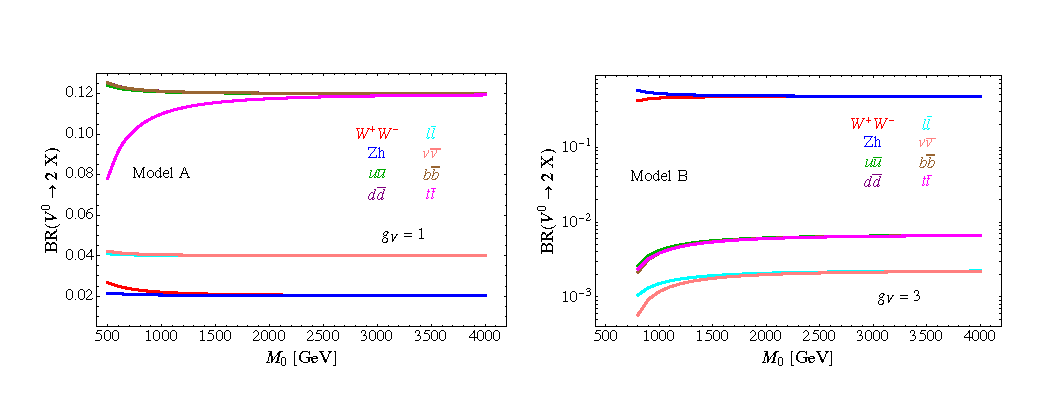
\includegraphics[width=0.99\textwidth]{figures/theory/hvtmodels.pdf}
\caption{Predicted branching fractions of a \PZpr for two explicit HVT models: Model  $\mathrm{A}_{g_V=1}$ (left) and model $\mathrm{B}_{g_V=3}$ (right)~\cite{Pappadopulo:2014qza}.}
\label{fig:theory:hvtBR}
\end{figure}
\clearpage

\section{Warped extra dimensions}
\label{sec:theory:wed}
Extra dimensional theories also offer solutions to the hierarchy problem. This thesis focuses on Randall-Sundrum (RS) warped extra dimensional scenarios~\cite{PhysRevLett.83.3370}. In RS models, a new curved spatial dimension $y$ is proposed, leading to a 5-dimensional space-time bounded by two (3+1)-dimensional planes, or \emph{branes}: the UV/Planck and the IR/TeV brane. The new metric now depends on the radius $r$ and the curvature factor $k$ of the new extra dimension, with
\begin{equation}
  ds^2=e^{-2ky}\eta_{\mu\nu}dx^{\mu}dx^{\nu}+dy^2; 0 < y < \pi R.
\end{equation}
Gravity is concentrated and relatively strong at the Planck brane at $y=0$, which is separated from us by the fifth dimension. Our observed four-dimensional reality and the Standard Model particles reside at the \TeV brane, at $y=\pi R$. Only gravity, transmitted through gravitons, is allowed to propagate through the warped 5D space-time (the "bulk") and is not confined to either brane. Figure~\ref{fig:theory:rs1} illustrates how the branes and the bulk are connected.
\begin{figure}[h!]
\centering
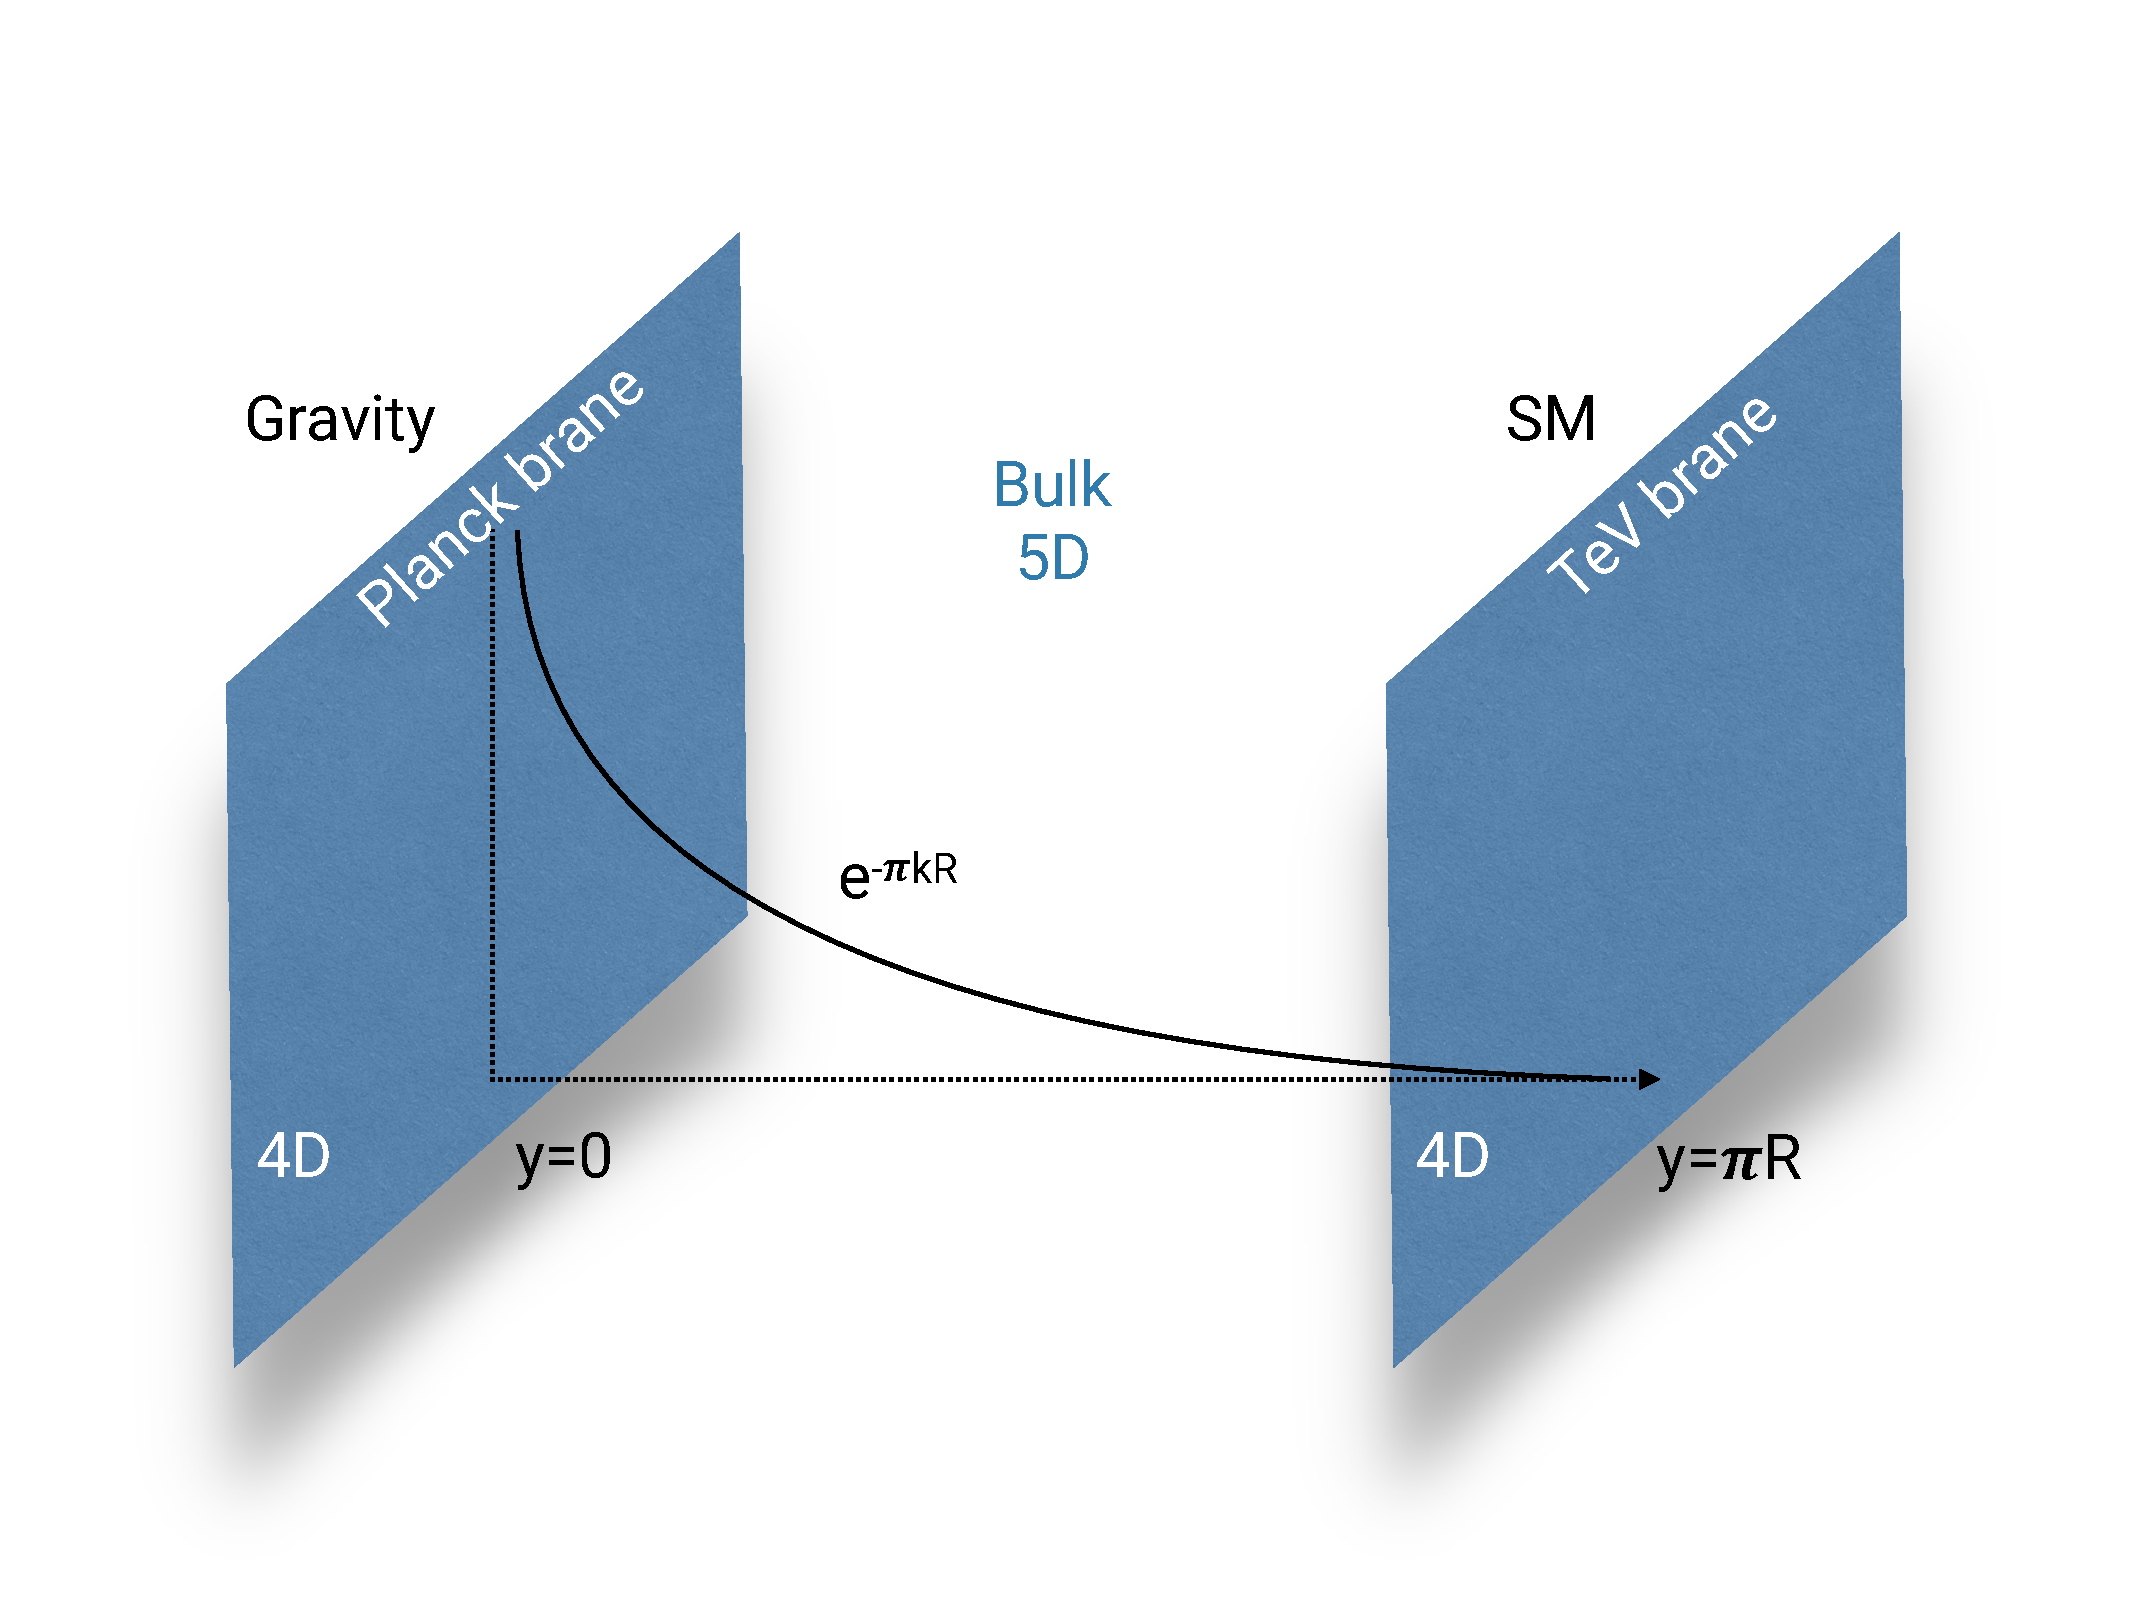
\includegraphics[width=0.49\textwidth]{figures/theory/rs1.pdf}
\caption{The RS model predicts an extra dimension where a 5D space-time stretches between two 4D branes: the Planck brane where gravity is concentrated, and the TeV brane where the SM particles are confined.}
\label{fig:theory:rs1}
\end{figure}
 Due to the warping, the Planck mass on the Planck brane gets reduced by a factor of $e^{-\pi kR}$ at the TeV brane, thereby solving the hierarchy problem. The Planck mass on the \TeV brane, which depends on the geometry of the extra dimension, becomes
\begin{equation}
  \bar{M}_{Pl}^2=V_1M_*^3,
  \end{equation} 
where $V_1$ is the volume of the 1 dimensional added warped dimension and $M_*^3$ is the 5D Planck mass.
One distinct prediction of the model, and a way in which we can test its validity, is the prediction of a tower of \TeV-scale excitations with spin-2, so called Kaluza-Klein states, that could be observed in high energy experiments. \newline
In this thesis, we are more interested in an alternative to the original RS model called the "bulk" scenario~\cite{PhysRevD.76.036006,Fitzpatrick:2007qr}. In this case, the Standard Model particles, besides the Higgs boson, are also allowed to propagate in the bulk. The light 1st and 2nd generation fermions are localized near the Planck brane, yielding small couplings to the Higgs boson that still resides at the \TeV brane, explaining their small masses. Similarly, the top quark is now located near the \TeV brane, resulting in a stronger Yukawa coupling to the Higgs boson. In addition, with the gravitons located near the \TeV brane and the fermions now residing near the Planck brane, the graviton coupling to fermions is strongly suppressed. SM gluons have a flat distribution throughout the bulk, making gluon-gluon production the dominant production channel of gravitons. Due to the weak vector bosons absorbing the Higgs degree of freedom in spontaneous symmetry breaking, their wave-functions fall off steeply near the \TeV brane, resulting in a coupling to the gravitons similar to that of the Higgs and the top. The only free parameters of the theory is the mass of the lightest KK graviton and the ratio $\tilde{k} = \frac{k}{\bar{M}_{Pl}}$, which controls the widths of the new resonances. The branching ratios of the Bulk Graviton is shown in Figure~\ref{fig:theory:bulk}.
\begin{figure}[h!]
\centering
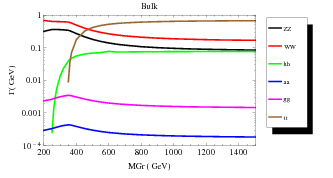
\includegraphics[width=0.49\textwidth]{figures/theory/BulkGravitonBR_tuomas.png}
\caption{Predicted branching fractions for a Bulk Graviton as a function of its mass.}
\label{fig:theory:bulk}
\end{figure}

